
	% ------------------------------------------------
\begin{frame}{Cálculo de ASV}
	\dificultyLevel{2}	
	Ahora queremos calcular ASV utilizando nuestra heurística:
	\only<1>{$$\assym_{M,e,\Pr}(x_i) = \heuristicASVFormula$$ } 
	\only<2>{$$\assym_{M,e,\Pr}(x_i) =\frac{1}{|\topo(G)|} \sum_{\alert{\equivalenceClass \in eqCl(G, x_i)}} (\charactheristicFunction(\toOr_{<i} \cup \{x_i\}) - \charactheristicFunction(\toOr_{<i})) * |\equivalenceClass|$$
		
		¿Cómo obtenemos las clases de equivalencia? }
	
	\end{frame}
	
\begin{comment}
		\item Primero necesitamos obtener el conjunto de clases de equivalencia $eqCl(G,x_i)$ y sus tamaños.
	\item Luego vamos a elegir un representante  por clase para evaluar la sumatoria.
	
	% ------------------------------------------------
	\begin{frame}[fragile]{Solución Naive}
		\dificultyLevel{3}
		\begin{algorithm}[H]
			\caption{NaiveEquivClasses($G$, $x_i$)} \label{alg:naiveAlgorithm}
			\begin{enumerate}
				\item $\mathit{orders} \leftarrow$ generarTodosLosOrdenesTopologicos($G$)
				\item Inicializar diccionarios \texttt{classes} y \texttt{classesSizes}
				\item Para cada $\pi \in \mathit{orders}$:
				\begin{enumerate}
					\item $U_{\pi} \leftarrow$ nodos no relacionados antes de $x_i$ en $\pi$
					\item Agregar $\pi$ a \texttt{classes}[$U_{\pi}$]
				\end{enumerate}
				\item Para cada clase $C$ en \texttt{classes}:
				\begin{enumerate}
					\item $\mathit{rep} \leftarrow$ first(\texttt{classes}[C])
					\item $\mathit{size} \leftarrow$ |\texttt{classes}[C]|
					\item \texttt{classesSizes}[$U_{\pi}$] $\leftarrow (rep, size, C)$
				\end{enumerate}
			\end{enumerate}
		\end{algorithm}
		\vspace{1ex}
		\textbf{Complejidad:} $O(n!)$ en el peor caso (todos los órdenes posibles).
	\end{frame}
\end{comment}

\begin{frame}{Solución Naive}
	\dificultyLevel{2}
	\begin{itemize}[<+- | alert@+>]
		\item \textbf{Generar todos los órdenes} topológicos $\mathit{orders}=\topo(G)$.
		\item Agrupar cada $\pi\in\mathit{orders}$ según 
		$U_\pi=$, sus nodos no relacionados antes de $x_i$.
		\item Para cada grupo $U_\toOr$, guardar un representante y su tamaño.
		\item \textbf{Complejidad:} $O(n!)$ en el peor caso.
	\end{itemize}
\end{frame}
	
	% ------------------------------------------------
	\begin{frame}{Algoritmo Recursivo}
	\dificultyLevel{2}
		\begin{itemize}[<+- | alert@+>]
			\item Etiquetar $G$ como:
			\begin{enumerate}
				\item Ancestros $A$ de $x_i$.
				\item Descendientes $D$ de $x_i$.
				\item Árboles no relacionados (raíces $UR$).
			\end{enumerate}
			\item Paso 1: calcular las clases de equivalencia para todos los subárboles no relacionados.
			\item Paso 2: fusionar los resultados obtenidos con $A$ y $D$.
		\end{itemize}
	\end{frame}
	
	% ------------------------------------------------
	\begin{frame}{Ejemplo: Grafo Etiquetado}
	\dificultyLevel{2}
		\begin{figure}[H]
			\centering
			 \begin{tikzpicture}[scale=.5, transform shape, 
				unrelated/.style={circle, draw=red},
				ancestor/.style={circle, draw=blue},
				]
				\node[text=blue, font=\Large] at (-5, 0) {Ancestros};
				\node[text=teal, font=\Large] at (-5, -0.5) {Descendientes};
				\node[text=red, font=\Large] at (-5, -1) {No relacionados};        
				
				% ---- NODOS ----
				
				\node[ancestor] (a1) at (0, 0) {$a_1$};
				\node[unrelated] (u1) at (-1, -2) {$u_1$};
				\node[ancestor] (a2) at (1, -2) {$a_2$};
				
				\drawUnrelatedTree{u2}{-1}{-4}{$u_2$}
				\node[ancestor] (a3) at (1, -4) {$a_3$};
				\node[unrelated] (u3) at (3, -4) {$u_3$};
				
				\drawUnrelatedTree{u4}{0}{-7}{$u_4$}
				\node[ancestor] (a4) at (3, -6) {$a_4$};
				
				\node[nodo, font=\Large] (xi) at (3, -8) {$x_i$};
				
				\drawUnrelatedTree{r1}{6}{0}{$u_5$} 
				\drawUnrelatedTree{r2}{10}{0}{$u_6$} 
				
				\node[draw=none, fill=none] (hi) at (3, -10) {};
				
				
				\path [->] (a1) edge[arista]  (u1);
				\path [->] (a1) edge[arista]  (a2);
				
				\path [->] (a2) edge[arista]  (u2);
				\path [->] (a2) edge[arista]  (a3);
				\path [->] (a2) edge[arista]  (u3);
				
				\path [->] (a3) edge[arista]  (u4);
				\path [->] (a3) edge[arista]  (a4);
				
				\path [->] (a4) edge[arista]  (xi);      
				\path [->, teal] (xi) edge[arista,  decorate, decoration={snake, amplitude=.4mm, segment length=4mm, post length=1mm}] node[right, font=\Large] {descendientes de $x_i$} (hi);
			\end{tikzpicture}
			\caption*{Digrafo etiquetado en base a $x_i$: Ancestros (azul), Descendientes (verde), No relacionados (rojo)}
			\label{fig:ASV_forest_example}
		\end{figure}
	\end{frame}
	
	% ————————————————————————
	% 1) Empezamos sólo con el subárbol b₁ (u₂ en tu código)
	% ————————————————————————

	\begin{frame}{Subárbol $u_2$}
		\dificultyLevel{3}
		\begin{figure}[H]
			\centering
			\begin{tikzpicture}[
				scale=.8, transform shape,
				unrelated/.style={circle,draw=red}
				]
				% Subárbol b₁
				\drawUnrelatedTreeLarge{u2}{0}{0}{$u_2$}
			\end{tikzpicture}
			\caption*{Subárbol aislado de nodos no relacionados}
		\end{figure}
	\end{frame}
	
	% ————————————————————————
	% 2) Todos los subárboles y flechas de combinación (bidireccional)
	% ————————————————————————
	\begin{frame}{Paso 1: Combinación de subárboles}
		\dificultyLevel{3}
		\begin{figure}[H]
			\centering
			\begin{tikzpicture}[
				scale=.8, transform shape,
				unrelated/.style={circle,draw=red}
				]
				% Los cuatro subárboles independientes
				\drawUnrelatedTreeLarge{u2}{-4}{0}{$u_2$}
				\drawUnrelatedTreeLarge{u4}{-1}{0}{$u_4$}
				\drawUnrelatedTreeLarge{r1}{2}{0}{$u_5$}
				\drawUnrelatedTreeLarge{r2}{5}{0}{$u_6$}
				
				% Un único arco con cabezas en ambas puntas
				\path[<->, thick] (u2) edge[bend left=20] (u4);
				\path[<->, thick] (u4) edge[bend left=20] (r1);
				\path[<->, thick] (r1) edge[bend left=20] (r2);
			\end{tikzpicture}
			\caption*{Podemos combinar estos subárboles, ya que no hay restricciones entre los mismos}
		\end{figure}
	\end{frame}

	
	% ————————————————————————
	% 3) Agregamos ancestros y descendientes y mostramos el merge
	% ————————————————————————
\begin{frame}{Paso 2: Fusión con ancestros y descendientes}
	\dificultyLevel{3}
	\begin{figure}[H]
		\centering
		\begin{tikzpicture}[
			scale=.5, transform shape,
			ancestor/.style={circle,draw=blue,minimum size=1cm,inner sep=2pt,font=\Large},
			xinode/.style  ={circle,draw=teal,minimum size=1.2cm,inner sep=2pt,font=\LARGE},
			mySnake/.style ={decorate,decoration={snake,amplitude=0.4mm,segment length=4mm,post length=1mm}}
			]
			% 1) Los subárboles (siguen igual)
			\drawUnrelatedTreeLarge{u2}{-4}{0}{$u_2$}
			\drawUnrelatedTreeLarge{u4}{-1}{0}{$u_4$}
			\drawUnrelatedTreeLarge{r1}{2}{0}{$u_5$}
			\drawUnrelatedTreeLarge{r2}{5}{0}{$u_6$}
			
			% 2) Ancestros (azul, más grandes)
			\node[ancestor] (a1) at (-4,2) {$a_1$};
			\node[ancestor] (a2) at (-1,2) {$a_2$};
			\node[ancestor] (a3) at (2,2)  {$a_3$};
			\node[ancestor] (a4) at (5,2)  {$a_4$};
			
			% 3) Descendiente x_i (círculo más grande y flecha “wiggly”)
			\node[xinode] (xi) at (0,-6) {$x_i$};
			\node[draw=none] (hi) at (0,-8) {};
			
			% ➤ Flechas de merge con ancestros
			\path[->, thick, blue] (a1) edge (u2);
			\path[->, thick, blue] (a2) edge (u4);
			\path[->, thick, blue] (a3) edge (r1);
			\path[->, thick, blue] (a4) edge (r2);
			
			% ➤ Flecha wiggly de descendientes
			\path[->, thick, teal]
			(xi) edge[mySnake]
			node[right,font=\Large] {descendientes de $x_i$} (hi);
		\end{tikzpicture}
		\caption*{Los ancestros tienen dependencias con los subárboles y los descendientes son libres}
	\end{figure}
\end{frame}
	
\begin{frame}{Restricciones en grafo etiquetado}
	\dificultyLevel{2}
	\begin{figure}[H]
		\centering
		\begin{tikzpicture}[scale=.5, transform shape, 
			unrelated/.style={circle, draw=red},
			ancestor/.style={circle, draw=blue},
			]
			\node[text=blue, font=\Large] at (-5, 0) {Ancestros};
			\node[text=teal, font=\Large] at (-5, -0.5) {Descendientes};
			\node[text=red, font=\Large] at (-5, -1) {No relacionados};        
			
			% ---- NODOS ----
			
			\node[ancestor] (a1) at (0, 0) {$a_1$};
			\node[unrelated] (u1) at (-1, -2) {$u_1$};
			\node[ancestor] (a2) at (1, -2) {$a_2$};
			
			\drawUnrelatedTree{u2}{-1}{-4}{$u_2$}
			\node[ancestor] (a3) at (1, -4) {$a_3$};
			\node[unrelated] (u3) at (3, -4) {$u_3$};
			
			\drawUnrelatedTree{u4}{0}{-7}{$u_4$}
			\node[ancestor] (a4) at (3, -6) {$a_4$};
			
			\node[nodo, font=\Large] (xi) at (3, -8) {$x_i$};
			
			\drawUnrelatedTree{r1}{6}{0}{$u_5$} 
			\drawUnrelatedTree{r2}{10}{0}{$u_6$} 
			
			\node[draw=none, fill=none] (hi) at (3, -10) {};
			
			
			\path [->] (a1) edge[arista]  (u1);
			\path [->] (a1) edge[arista]  (a2);
			
			\path [->] (a2) edge[arista]  (u2);
			\path [->] (a2) edge[arista]  (a3);
			\path [->] (a2) edge[arista]  (u3);
			
			\path [->] (a3) edge[arista]  (u4);
			\path [->] (a3) edge[arista]  (a4);
			
			\path [->] (a4) edge[arista]  (xi);      
			\path [->, teal] (xi) edge[arista,  decorate, decoration={snake, amplitude=.4mm, segment length=4mm, post length=1mm}] node[right, font=\Large] {descendientes de $x_i$} (hi);
		\end{tikzpicture}
		\caption*{Digrafo etiquetado en base a $x_i$: Ancestros (azul), Descendientes (verde), No relacionados (rojo)}
		\label{fig:ASV_forest_example}
	\end{figure}
\end{frame}
	
\begin{comment}
		\begin{frame}{Intuición de \texttt{unrEqCl}}
		\dificultyLevel{3}
		\begin{itemize}[<+- | alert@+>]
			\item Para calcular las clases de los árboles no relacionados vamos a seguir un razonamiento similar al de calcular la cantidad de clases. 
			\item Descomponemos un subárbol en subproblemas: cada nodo $node$ reutiliza clases de sus hijos.
			\item \textbf{Caso base (hojas)}: solo dos configuraciones posibles, puede estar a la izquierda o la derecha. 
			\item \textbf{Caso recursivo}: combinamos los resultados de los hijos utilizando la función $union$. 
			\item \texttt{union} combina distintas clases de equivalencia, si quieren saber como lo hace pueden leer la tesis $\heartsuit$
		\end{itemize}
	\end{frame}
	
	\item \textbf{Caso recursivo}: para cada combinación \(mix\) de clases hijas,
	\begin{itemize}
		\item Se coloca al nodo a la izquierda y se combinan todos los resultados de sus hijos:  \texttt{union(mix, $node_{left}$)}.
		\item Se coloca al nodo a la derecha y se colocan todos sus hijos a la derecha:  \texttt{union(mix, $node_{left}$)}.
	\end{itemize}
\end{comment}
	
\begin{frame}{Fórmulas amenas}
	\dificultyLevel{4}	
	\begin{align*}\label{formula:union}
		&\union(((repEC_1, lTopo_1, rTopo_1), ...., (repEC_{|n|}, lTopo_{|n|}, rTopo_{|n|})), n_t) = \\
		&(class,l,r)\\ 
		&class = \bigcup_{j=1}^{|n|} repEC_j \cup \set{n_t} \\
		&l = \binom{\sum_{i=1}^{|n|} |L(repEC_i)|}{|L(repEC_1)|, \ldots, |L(repEC_{|n|})|} \prod_{i=1}^{|n|} lTopo_i, \\ 
		&r=\binom{\sum_{i=1}^{|n|} |R(repEC_i)|}{|R(repEC_1)|, \ldots, |R(repEC_{|n|})|} \prod_{i=1}^{|n|} rTopo_i 
	\end{align*}
\end{frame}

\begin{frame}{Más fórmulas amenas}
	\dificultyLevel{5}	
	\scriptsize
	\[
	\leftPossibleOrders(p,i,npa) = 
	\begin{cases} 
		\begin{aligned}
			\binom{ cp(i, npa)}{npa[1], \ldots, npa[i]} 
		\end{aligned} & \text{if $|A|=i$} \\
		\begin{aligned}
			&\sum_{toFill=p}^{p+cp(i,npa)} \sum_{comb \in pb(toFill-p-1,i, npa)} \Big(\binom{ sum(comb)}{comb_1, \ldots, comb_i} \\
			&  \cdot \leftPossibleOrders(toFill,i+1,hp(comb, npa)\Big)
		\end{aligned}
		& \text{otherwise}
	\end{cases}
	\]
\end{frame}

\begin{comment}
		% ------------------------------------------------
	\begin{frame}[fragile]{Clases en Árboles No Relacionados}
		\dificultyLevel{4}
		\begin{itemize}
			\item \textbf{Recordemos:} $UR$ = raíces de subárboles sin relación causal con $x_i$. 
			\item La función devuelve un conjunto de tuplas de la forma $(\equivalenceClassRep, leftTopos, rightTopos)$.
		\end{itemize}
		
		\pause 
		\begin{align*}\label{formula:unrelated_equiv_classes}
			\unrEqCl(n) = 
			\begin{cases} 
				\set{(\set{n_l}, 1, 1), (\set{n_r},1,1)} & \text{si $n$ es una hoja} \\[1ex]
				\begin{aligned}
					&\left( \bigcup_{\forall mix \in \unrEqCl(n_1) \times \dots \times \unrEqCl(n_{|n|})} \hspace{-5em} \union(mix,n_{left})\right) \\
					&\cup \union(right,n_{right})
				\end{aligned} & \text{cc}
			\end{cases}
		\end{align*}
	\end{frame}
\end{comment}

\begin{comment}
		
		Fórmula de eqClassSizes:
			Recorremos todas las combinaciones de clases de subárboles (UR).
			Para cada combinación, fusionamos con ancestros y descendientes.
			Calculamos el tamaño de cada clase como \#órdenes posibles.
			El resultado es el conjunto de todas las clases y sus tamaños.
			Fórmula de eqClassSizes: Contar que luego combinamos ambos resultados para ver la cantidad total de órdenes
		Intuición eqClass:
			Construye un orden topológico que respeta todas las dependencias internas.
		Left orders: 
			Al recorrer recursivamente, se reutilizan combinaciones parciales (DP). Puesto que podemos llegar a la misma configuración por varios caminos.
		
		\begin{frame}{Fórmula de \eqClassSizes}
			\dificultyLevel{3}
			\only<1>{%
				Habiendo realizado estos cálculo estamos listos para definir nuestra fórmula para el \textbf{conjunto de clases de equivalencia y sus tamaños}.
				\[
				\eqClassSizes(G,x_i) = \,\cdots
				\]
				
				%\textbf{Definición:} 		\begin{itemize}			\item $UR$: raíces de subárboles \alert{no relacionados} con $x_i$.		\end{itemize}
			}
			\only<2>{%
				\[
				\eqClassSizes(G,x_i)
				= \bigcup_{\displaystyle mix\in
					\prod_{j=1}^{|UR|}\unrEqCl(ur_j)} \,\cdots
				\]
				\vspace{1em}
				\textbf{Nota:}
				\begin{itemize}
					\item Cada $mix$ es una combinación (producto cartesiano) de 
					las clases de cada $ur_j\in UR$.
				\end{itemize}
			}
			\only<3>{%
				\[
				\eqClassSizes(G,x_i)
				= \bigcup_{mix}
				\Bigl(\,eqCl(A,D,mix),\,\eqClassSize(A,D,mix)\Bigr)
				\]
				\vspace{1em}
				\textbf{¿Qué hace?}
				\begin{itemize}
					\item $eqCl(A,D,mix)$ fusiona \alert{ancestros $A$}, 
					\alert{descendientes $D$} y la combinación $mix$.
				\end{itemize}
			}
			\only<4->{%
				\[
				\eqClassSizes(G,x_i)
				= \hspace{-3em} \bigcup_{mix\in\prod_{j=1}^{|UR|}\unrEqCl(ur_j)} \hspace{-3em}
				\Bigl(eqCl(A,D,mix),\,\eqClassSize(A,D,mix)\Bigr)
				\]
				\vspace{1em}
				\textbf{Componentes finales:}
				\begin{itemize}
					\item<4-> $eqCl(A,D,mix)$: representa la clase resultante tras fusionar.
					\item<5-> $\eqClassSize(A,D,mix)$: cantidad de órdenes topológicos de esa clase.
				\end{itemize}
			}
			
		\end{frame}
		
	
		\only<6->{%
		\vspace{1em}
		\textbf{Resumen:}
		\begin{itemize}
			\item<6-> Recorremos \alert{todas} las combinaciones de clases de subárboles (UR).
			\item<7-> Para cada combinación, fusionamos con ancestros y descendientes.
			\item<8-> Calculamos el tamaño de cada clase como \#órdenes posibles.
			\item<9-> El resultado es el conjunto de todas las clases y sus tamaños.
		\end{itemize}
	}
\end{comment}

\begin{comment}
	% ------------------------------------------------------------------------
	\begin{frame}{Intuición de $\;eqCl(A,D,mix)\;$}
		\dificultyLevel{2}
		\begin{itemize}
			\item La función $eqCl(A,D,mix)$ “fusiona” tres componentes:
			\begin{enumerate}
				\item<2-> Los \alert{ancestros} $A$ de $x_i$, que deben aparecer antes.
				\item<3-> La \alert{combinación $mix$}, la cual define que nodos están a la izquierda y cuáles a la derecha. 
				\item<4-> Los \alert{descendientes} $D$ de $x_i$, que deben aparecer después.
			\end{enumerate}
			%\item<5-> En esencia, construye un orden topológico que respeta todas las dependencias internas.
		\end{itemize}
	\end{frame}
	
	\item Partimos de una combinación $mix$, que agrupa las clases de cada subárbol unrelated:
		\[
		mix \;\in\; \prod_{j=1}^{|UR|}\unrEqCl(ur_j).
		\]
\end{comment}

\begin{comment}
	
	% ------------------------------------------------------------------------
	\begin{frame}{Cálculo de $\eqClassSize(A,D,mix)$}
		\dificultyLevel{2}
		\begin{block}{Ancestros: función \texttt{leftOrders}}
			\begin{itemize}
				\item Inserta recursivamente cada ancestro $a\in A$ en los huecos válidos.
				\item Cuenta cuántos órdenes parciales respetan las dependencias.
				\item Resultado: número de formas de intercalar los nodos unrelated \alert{antes} de $x_i$ con los ancestros.
			\end{itemize}
		\end{block} 
		\pause
		\begin{block}{Descendientes: conteo combinatorio}
			\begin{itemize}
				\item No hay dependencias entre $D$ y $UR$ tras $x_i$.
				\item Por lo tanto podemos combinar los elementos de ambos conjuntos libremente, al igual que al usar $union$. 
				%\item Cada clase $mix$ aporta $R(mix)$ nodos a la derecha.
				%\item Luego la cuenta es meramente hacer la combinatoria entre estos dos conjuntos. 
				
			\end{itemize}
		\end{block}
	\end{frame}
	
	% ------------------------------------------------------------------------
	\begin{frame}[fragile]{Algoritmo \texttt{leftOrders}}
		\dificultyLevel{4}
		\begin{algorithm}[H]
			\caption*{leftOrders($A$, $\textit{actual ancestor}$, $\textit{nodes to place}$, $position$)} \label{alg:leftOrdersAlgorithm}
			\begin{enumerate}
				\item Definimos donde colocar $\textit{actual ancestor}$ en base a $position$ y a cuántos nodos tenemos disponibles en $\textit{nodes to place}$, generando $\textit{new position}$.
				\item Luego seleccionamos cuántos nodos de cada unrelated tree vamos a usar para llenar todas las posiciones entre $position$ y $\textit{new position}$, generando $\textit{new nodes}$.
				\item Eliminamos los $\textit{new nodes}$ de los $\textit{nodes to place}$, puesto que ya los colocamos, actualizando nuestros nodos disponibles.
				\item Realizamos el llamado recursivo actualizando la posición, nuestros nodos disponibles y nuestro ancestro actual. 
			\end{enumerate}
		\end{algorithm}
	\end{frame}
	
	% ------------------------------------------------------------------------
	\begin{frame}{Intuición de \texttt{leftOrders}}
		\dificultyLevel{3}
		\begin{itemize}[<+- | alert@+>]
			\item Recorre los ancestros en orden.
			\item En cada paso reparte los nodos no relacionados en los “huecos” antes del ancestro:
			\[
			[\,\underbrace{\;\; }_{a_0}\;|\;\underbrace{\;\; }_{a_1}\;|\;\dots\;|\;\underbrace{\;\; }_{a_{|A|}}\;]
			\]
			%\item Al recorrer recursivamente, se reutilizan combinaciones parciales (DP). Puesto que podemos llegar a la misma configuración por varios caminos.
		\end{itemize}
	\end{frame}
	
	% ------------------------------------------------------------------------
	\begin{frame}{Iteración: Posición de Ancestros}
		\dificultyLevel{3}
		\begin{figure}[ht]
			\centering
			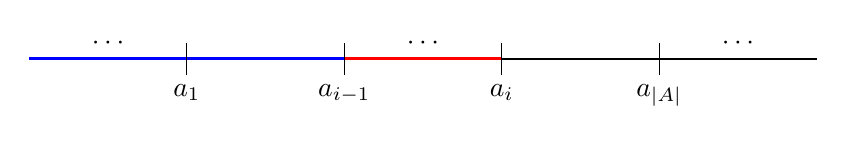
\begin{tikzpicture}
				\draw[thick] (0,0) -- (10,0);
				\draw[blue,very thick] (0,0) -- (4,0);
				\draw[red,very thick]  (4,0) -- (6,0);
				\foreach \x/\y in {2/$a_1$,4/$a_{i-1}$,6/$a_i$,8/$a_{|A|}$} {
					\draw (\x,0.2) -- (\x,-0.2);
					\node[below] at (\x,-0.2){\y};
				}
				\node at (1,0.2){$\cdots$};
				\node at (5,0.2){$\cdots$};
				\node at (9,0.2){$\cdots$};
			\end{tikzpicture}
			\caption*{Paso $i$: Azul = ancestros ya colocados; Rojo = espacio de longitud $newPosition- position$.}
			\label{fig:leftOrdersIterationTopoOrder}
		\end{figure}
		%\begin{itemize}[<+- | alert@+>]		\item El tramo rojo marca cuántas posiciones quedan para nodos no relacionados.		\item El algoritmo itera todos los posibles “offsets” $toFill$ en ese intervalo.	\end{itemize}
	\end{frame}
	
	% ------------------------------------------------------------------------
	
\end{comment}

% ------------------------------------------------------------------------
	
% ------------------------------------------------------------------------
\begin{comment}
	
	\begin{frame}{Left orders: La fórmula más amena}
		\dificultyLevel{5}	
		\scriptsize
		\[
		\leftPossibleOrders(p,i,npa) = 
		\begin{cases} 
			\begin{aligned}
				\binom{ cp(i, npa)}{npa[1], \ldots, npa[i]} 
			\end{aligned} & \text{if $|A|=i$} \\
			\begin{aligned}
				&\sum_{toFill=p}^{p+cp(i,npa)} \sum_{comb \in pb(toFill-p-1,i, npa)} \Big(\binom{ sum(comb)}{comb_1, \ldots, comb_i} \\
				&  \cdot \leftPossibleOrders(toFill,i+1,hp(comb, npa)\Big)
			\end{aligned}
			& \text{otherwise}
		\end{cases}
		\]
	\end{frame}
	
	
	% ------------------------------------------------------------------------
	\begin{frame}{Iteración: Nodos Disponibles}
		\dificultyLevel{3}
		\begin{figure}[H]
			\centering
			\begin{tikzpicture}[scale=.45, transform shape, 
				unrelated/.style={circle, draw=red},
				ancestor/.style={circle, draw=blue},
				wiggly/.style={decorate, decoration={snake, amplitude=.2mm, segment length=2mm}}  % Define wiggly line style
				]
				
				\node[draw=none, fill=none] (a1) at (0, 0) {};
				\node[ancestor] (a2) at (1, -2) {$a_{i-1}$};
				
				\drawUnrelatedTreeWithTag{u2}{-1}{-4}{$u_{i-1}$}{orange}{Available nodes: npa[i-1]}
				
				\drawUnrelatedTree{u4}{0}{-7}{$u_{i}$}
				\node[ancestor] (a3) at (3, -6) {$a_i$};
				
				\node[draw=none, fill=none] (xi) at (3, -8) {};
				
				\drawUnrelatedTreeWithTag{r1}{6}{0}{$u_5$}{orange}{Available nodes: npa[0]};
				\drawUnrelatedTreeWithColor{r2}{10}{0}{$u_6$}{orange};
				
				
				\path [->] (a1) edge[arista,  decorate, decoration={snake, amplitude=.4mm, segment length=4mm, post length=1mm}] (a2);
				
				\path [->] (a2) edge[arista]  (u2);
				\path [->] (a2) edge[arista]  (a3);
				
				\path [->] (a3) edge[arista]  (u4);
				\path [->] (a3) edge[arista,  decorate, decoration={snake, amplitude=.4mm, segment length=4mm, post length=1mm}] (xi);
			\end{tikzpicture}
			%\caption*{Los nodos pintados en naranja son los nodos disponibles para ser colocados en el paso $i$. Para cada conjunto de subárboles $npa$ (nodes to place) tiene la cantidad de nodos disponibles.}
			\label{fig:leftOrdersIterationGraph}
		\end{figure}
		\begin{itemize}
			\item Solo los nodos de $u_{i-1}$ pueden rellenar el hueco antes de $a_i$.
			%\item Tras fijar $a_i$, ampliamos el conjunto de nodos disponibles.
		\end{itemize}
	\end{frame}
	
	\begin{frame}{Cálculo de $\;\eqClassSize(A,D,mix)\;$}
		\dificultyLevel{2}
		Una vez conocidos:
		\begin{itemize}
			\item $N_{\mathrm{anc}} = \texttt{leftOrders}(A,mix)$ \quad (\# órdenes parciales con ancestros),
			\item $N_{\mathrm{desc}} = \displaystyle\binom{L+|D|}{|D|}$ \quad (\# colocaciones de descendientes),
		\end{itemize}
		\pause
		entonces el tamaño de la clase es el producto:
		\[
		\eqClassSize(A,D,mix)
		\;=\;
		N_{\mathrm{anc}}
		\;\times\;
		N_{\mathrm{desc}}.
		\]
		\pause 
		Así es cómo ya tenemos nuestras clases de equivalencia y sus tamaños, ahora sólo falta ver la \textbf{complejidad} de este algoritmo.
	\end{frame}
\end{comment}

\begin{frame}{Complejidad Temporal}
	\dificultyLevel{2}
	\small
	\begin{columns}[t]
		%---------------------------%
		\column{0.48\textwidth}
		\begin{block}{Complejidad de \unrEqCl }
			\begin{itemize}[<+- | alert@+>]
				\item Costo de \texttt{union}: $O(n)$.
				\item Cantidad de clases generadas: $\le |EC|$.
				\item Invocado en cada arból $\leq n$:
				\[
				O\bigl(n \times (n\cdot |EC|)\bigr)
				= O\bigl(n^2\,|EC|\bigr).
				\]
			\end{itemize}
		\end{block}
		
		%---------------------------%
		\column{0.48\textwidth}
				\only<2> {
		\begin{mydefinition}[Cantidad de clases de equivalencia]
				En vez de usar $\#clases$ vamos a usar $|EC|$ = Ezequiel Companeetz = Equivalence Classes.
			\end{mydefinition}
		}
		\visible<3->{%
			\begin{block}{Algoritmo Completo}
				\begin{itemize}[<+- | alert@+>]
					\item Fusionar clase no relacionada con ancestros y descendientes: $O(n^5\,|EC|^2)$ por clase.
					\item Clases no relacionadas: $O\bigl(n^2\,|EC|\bigr)$.
					\item Total:
		            \begin{align*}
							&O(n^2\,|EC|) + |EC|\times O(n^5\,|EC|^2) \\
							&= O(n^5\,|EC|^3).
					\end{align*}
				\end{itemize}
		\end{block}}
	\end{columns}
\end{frame}



	
